\documentclass{article}
\usepackage{tikz}
\begin{document}
\begin{center}
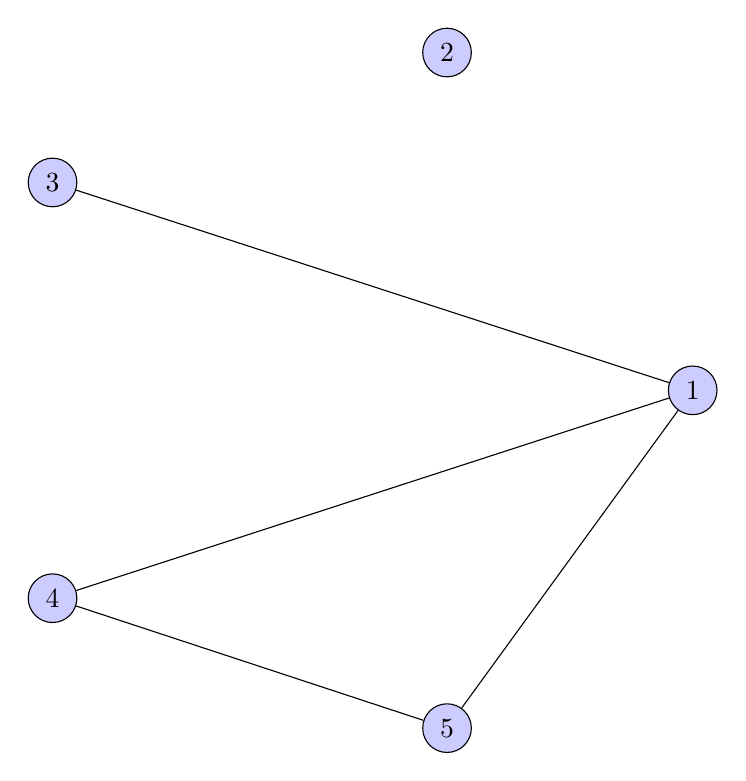
\begin{tikzpicture}[scale=3, every node/.style={circle, draw, fill=blue!20}]
\node (N0) at (1.50,0.00) {1};
\node (N1) at (0.46,1.43) {2};
\node (N2) at (-1.21,0.88) {3};
\node (N3) at (-1.21,-0.88) {4};
\node (N4) at (0.46,-1.43) {5};
\draw (N0) -- (N4);
\draw (N0) -- (N3);
\draw (N0) -- (N2);
\draw (N3) -- (N4);
\end{tikzpicture}
\end{center}
\end{document}